\documentclass[11pt,openany]{article}

\input{algebra-preamble}
\usepackage{caption}
%Tikzpicture
\usepackage{tikz}
\usepackage{tikz-3dplot}
\usepackage{tikz-cd}
\usetikzlibrary{
	3d, % For 3D drawing
	angles,
	arrows,
	arrows.meta,
	backgrounds,
	bending,
	calc,
	decorations.pathmorphing,
	decorations.pathreplacing,
	fit,
	matrix,
	patterns,
	patterns.meta,
	positioning,
	quotes,
	shadows,
	shapes,
	shapes.geometric
}

\setstretch{1.25}
\begin{document}
\pagenumbering{arabic}
\begin{center}
	\huge\textbf{Equivalence Relations, Equivalence Classes,\\ Partitions, and Quotient Sets}\\
	\vspace{0.5em}
%	\Large\quad{대수학의 아름다움 서브-스터디}\\
	\vspace{0.5em}
	\normalsize{\today}\\
\end{center}

\section*{Cartesian Products / Set Products}
\begin{center}
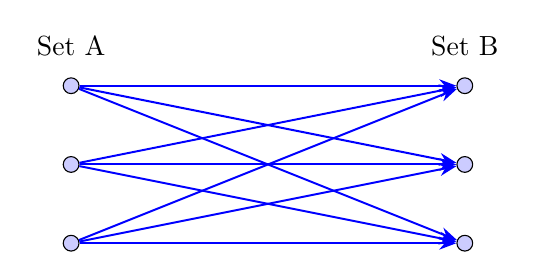
\begin{tikzpicture}\tikzset{set node/.style={circle, draw, fill=blue!20, minimum size=2mm, inner sep=0pt}}
	% Define the sets
	\node at (0,4.5) {Set A};
	\node at (5,4.5) {Set B};
	\node[set node] at (0,4) (a1) {};
	\node[set node] at (0,3) (a2) {};
	\node[set node] at (0,2) (a3) {};
	
	\node[set node] at (5,4) (b1) {};
	\node[set node] at (5,3) (b2) {};
	\node[set node] at (5,2) (b3) {};
	
	% Connect every node from set A to every node from set B
	\foreach \i in {1,2,3}
	\foreach \j in {1,2,3}
	\draw[-Stealth, blue, line width=.25mm] (a\i) -- (b\j);
\end{tikzpicture}
\end{center}
\begin{example*}
	If $A=\set{1,2}$ and $B=\set{x,y}$, then: \[
	A\times B=\set{(1,x),(1,y),(2,x),(2,y)}
	\]
\end{example*}
\begin{definition*}
	Let $A$ and $B$ are sets. \[
	A\times B:=\set{(a,b)\mid a\in A\ \text{and}\ b\in B}
	\]
\end{definition*}

\section*{Relations}
\begin{center}
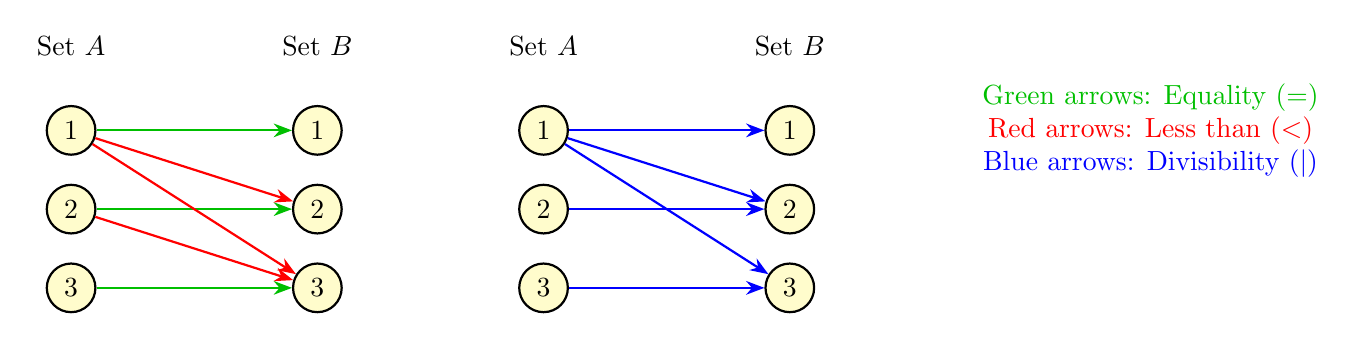
\begin{tikzpicture}[>=Stealth, node distance=1cm and 2cm]
	% Styles for sets, elements, and annotations
	\tikzset{
		set node/.style={rectangle, draw, thick, fill=orange!20, minimum size=5mm, align=center},
		relation arrow/.style={->, thick, #1},
		element node/.style={circle, draw, thick, fill=yellow!20, minimum size=5mm},
		highlight/.style={draw, thick, dotted, inner sep=3pt}
	}
	
	% Define nodes for elements
	\node[] (a) {Set $A$};
	\node[right=of a] (b) {Set $B$};
	\node[element node, below=0.5cm of a] (a1) {1};
	\node[element node, below of=a1] (a2) {2};
	\node[element node, below of=a2] (a3) {3};
	\node[element node, below=0.5cm of b] (b1) {1};
	\node[element node, below of=b1] (b2) {2};
	\node[element node, below of=b2] (b3) {3};
	
	% Draw relations
	% Equality relation
	\foreach \x in {1, 2, 3}
	\draw[relation arrow=green!75!black] (a\x) -- (b\x);
	%		% Less than relation
	\draw[relation arrow=red] (a1) -- (b2);
	\draw[relation arrow=red] (a1) -- (b3);
	\draw[relation arrow=red] (a2) -- (b3);
	\begin{scope}[xshift=6cm]
		% Define nodes for elements
		\node[] (aa) {Set $A$};
		\node[right=of aa] (bb) {Set $B$};
		\node[element node, below=0.5cm of aa] (a4) {1};
		\node[element node, below of=a4] (a5) {2};
		\node[element node, below of=a5] (a6) {3};
		\node[element node, below=0.5cm of bb] (b4) {1};
		\node[element node, below of=b4] (b5) {2};
		\node[element node, below of=b5] (b6) {3};% Annotations for explanations
		% Divisibility relation
		\draw[relation arrow=blue] (a4) -- (b4);
		\draw[relation arrow=blue] (a4) -- (b5);
		\draw[relation arrow=blue] (a4) -- (b6);
		\draw[relation arrow=blue] (a5) -- (b5);
		\draw[relation arrow=blue] (a6) -- (b6);
		\node[align=center, right=2cm of b4] (text) {
			%				\textbf{Relations}\\
			\textcolor{green!75!black}{Green arrows: Equality ($=$)}\\
			\textcolor{red}{Red arrows: Less than ($<$)}\\
			\textcolor{blue}{Blue arrows: Divisibility ($\mid$)}
		};
	\end{scope}
\end{tikzpicture}
\end{center}
\begin{definition*}
	Let $A$ and $B$ are sets. A \textbf{relation} $\mathcal{R}$ from $A$ to $B$ is a \emph{subset} of the Cartesian Product $A\times B$: \[
	\mathcal{R}\subseteq A\times B
	\]
\end{definition*}
\begin{notation*}
	$$(a,b)\in\mathcal{R}\subseteq A\times B\iff a\mathrel{\mathcal{R}}b.$$ For example, $a=b\iff (a,b)\in\ =$
\end{notation*}

\section*{Equivalence Relations}
\begin{center}
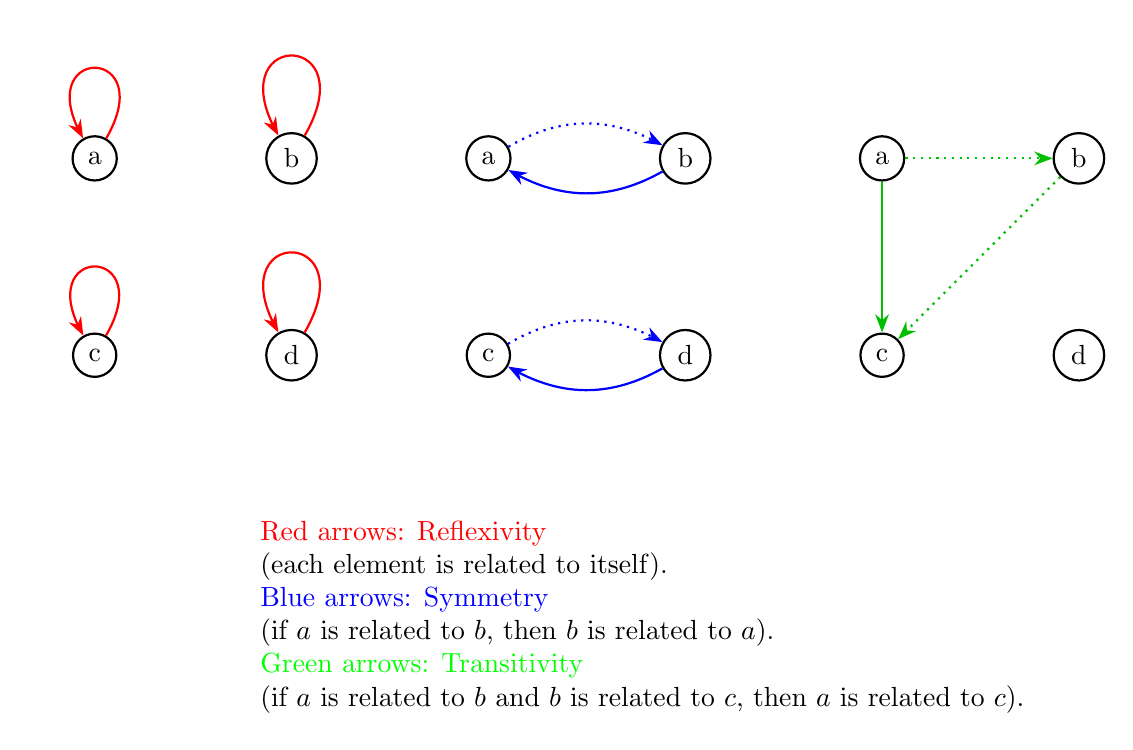
\begin{tikzpicture}[>=Stealth, node distance=2.5cm, thick, main/.style = {draw, circle}]
	% Define styles
	\tikzset{
		reflexive/.style={->, loop, looseness=12, in=120, out=60, red},
		symmetric/.style={->, blue, bend left},
		transitive/.style={->, green!75!black}
	}
	
	% Nodes
	\node[main] (a) {a};
	\node[main] (b) [right of=a] {b};
	\node[main] (c) [below of=a] {c};
	\node[main] (d) [right of=c] {d};
	
	% Edges
	% Reflexivity
	\draw[reflexive] (a) to (a);
	\draw[reflexive] (b) to (b);
	\draw[reflexive] (c) to (c);
	\draw[reflexive] (d) to (d);
	\begin{scope}[xshift=5cm]
		% Nodes
		\node[main] (a2) {a};
		\node[main] (b2) [right of=a2] {b};
		\node[main] (c2) [below of=a2] {c};
		\node[main] (d2) [right of=c2] {d};
		
		% Symmetry
		\draw[dotted,symmetric] (a2) to (b2);
		\draw[symmetric] (b2) to (a2);
		\draw[dotted,symmetric] (c2) to (d2);
		\draw[symmetric] (d2) to (c2);
	\end{scope}
	
	\begin{scope}[xshift=10cm]
		% Nodes
		\node[main] (a3) {a};
		\node[main] (b3) [right of=a3] {b};
		\node[main] (c3) [below of=a3] {c};
		\node[main] (d3) [right of=c3] {d};
		
		% Transitivity
		\draw[dotted, transitive] (a3) to (b3);
		\draw[dotted, transitive] (b3) to (c3);
		\draw[transitive] (a3) to (c3); % Transitivity implied by a -> d and d -> b
	\end{scope}
	
	% Annotations
	\node[align=left, below right= of c] {
		%		\textbf{Equivalence Relation Properties:}\\
		\textcolor{red}{Red arrows: Reflexivity}\\ (each element is related to itself).\\
		\textcolor{blue}{Blue arrows: Symmetry}\\ (if \(a\) is related to \(b\), then \(b\) is related to \(a\)).\\
		\textcolor{green}{Green arrows: Transitivity}\\ (if \(a\) is related to \(b\) and \(b\) is related to \(c\), then \(a\) is related to \(c\)).
	};
\end{tikzpicture}
\end{center}
\begin{example*}Equality on $\Z$: \begin{itemize}
	\item $a\in \Z\implies a=a$;
	\item $a=b\implies b=a$;
	\item $a=b$ and $b=c$ $\implies a=c$.
\end{itemize}
%Modular $n$ on $\Z$: \begin{itemize}
%	\item $a\in \Z\implies a\equiv a\pmod{n}$;
%	\item $a\equiv b\pmod{n}\implies b\equiv a\pmod{n}$;
%	\item $a\equiv b\pmod{n}$ and $b\equiv c\pmod{n}$ $\implies a\equiv c\pmod{n}$.
%\end{itemize} Note that $a\equiv b\pmod{n}\overset{\text{def}}{\iff} n\mid a-b\overset{\text{def}}{\iff}\exists k\in\Z:kn=a-b$
\end{example*}
\begin{definition*}
	Given a set $A$, a relation $\mathcal{R}\subseteq A\times A$ is called an \textbf{equivalence relation} if it satisfies following properties: \begin{itemize}
		\item (Reflexivity) $a\in A\implies (a,a)\in{\mathcal{R}}$;
		\item (Symmetry) $(a,b)\in \mathcal{R}\implies (b,a)\in \mathcal{R}$;
		\item (Transitivity) $(a,b)\in\mathcal{R}\land (b,c)\in\mathcal{R}\implies (a,c)\in\mathcal{R}$.
	\end{itemize}
\end{definition*}

\section*{Equivalence Classes}
\begin{center}
\begin{minipage}{.48\textwidth}\adjustbox{scale=.75, center}{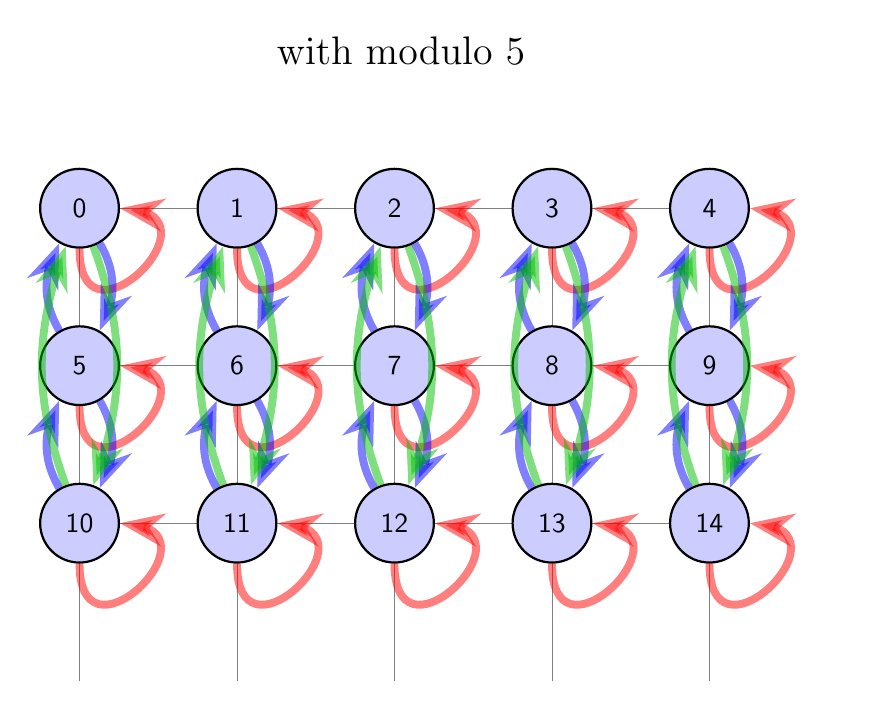
\begin{tikzpicture}[>=Stealth, thick, node distance=2 cm]
		% Styles for different components
		\tikzset{
			main node/.style={circle, draw, fill=blue!20, minimum size=1cm, font=\sffamily},
			class node/.style={ellipse, draw, thick, red, minimum height=2.5cm, minimum width=4cm, align=center},
			path/.style={->, thick, shorten <=2pt, shorten >=2pt},
			reflexive/.style={->, line width=1mm, loop, looseness=5, in=0, out=-90, red, opacity=.5},
			symmetric/.style={->, line width=1mm, blue, bend left, opacity=.5},
			transitive/.style={->, thick, green!75!black, bend left}
			label distance=3mm
		}
		
		% Nodes representing elements
		\node[main node] (0) {0};
		\node[main node] (1) [right of=0] {1};
		\node[main node] (2) [right of=1] {2};
		\node[main node] (3) [right of=2] {3};
		\node[main node] (4) [right of=3] {4};
		
		\node[main node] (5) [below of=0] {5};
		\node[main node] (6) [below of=1] {6};
		\node[main node] (7) [below of=2] {7};
		\node[main node] (8) [below of=3] {8};
		\node[main node] (9) [below of=4] {9};
		
		\node[main node] (10) [below of=5] {10};
		\node[main node] (11) [below of=6] {11};
		\node[main node] (12) [below of=7] {12};
		\node[main node] (13) [below of=8] {13};
		\node[main node] (14) [below of=9] {14};
		
		\node at (4,2) {\Large $\Z$ with modulo 5};
		
		\foreach \x in {0,1,2,...,14} {
			\draw[reflexive] (\x) to (\x);
		}
		
		\foreach \x/\y in {
			0/5, 5/10, 1/6, 6/11,
			2/7, 7/12, 3/8, 8/13,
			4/9, 9/14} {
			\draw[symmetric] (\x) to (\y);
			\draw[symmetric] (\y) to (\x);
		}
		
		\foreach \a/\b in {
			0/10, 1/11, 2/12, 3/13, 4/14} {
			\draw[->, line width=1mm, green!75!black, bend left=20pt, opacity=.5] (\a) to (\b);
			\draw[->, line width=1mm, green!75!black, bend left=20pt, opacity=.5] (\b) to (\a);
		}
		
		%	 Nodes for equivalence classes
		%			\node[class node, label={[red]above:Class $[1]$}, fit=(1)] {};
		%			\node[class node, label={[red]above:Class $[2, 3]$}, fit=(2) (3)] {};
		%			\node[class node, label={[red]above:Class $[4, 5]$}, fit=(4) (5)] {};
		
		% Connections showing relations (for illustration)
		%			\draw[path] (2) to[bend left] (3);
		%			\draw[path] (3) to[bend left] (2);
		%			\draw[path] (4) to[bend left] (5);
		%			\draw[path] (5) to[bend left] (4);
		
		% Annotations
		%	\node[align=center, below=3cm of 3, text width=12cm] {
			%		\large \textbf{Partition by Equivalence Relation}\\
			%		This diagram illustrates how an equivalence relation partitions a set into disjoint equivalence classes. Each class, outlined in red, contains elements that are equivalent under the relation.\\
			%		Arrows indicate specific relationships that define equivalence within classes. Classes $[2, 3]$ and $[4, 5]$ show internal symmetry, highlighting how elements within these groups are related to each other.
			%	};
		
		% Background grid as optional visual enhancement
		\begin{scope}[on background layer]
			\draw[style=help lines, step=2cm] (0,0) grid (8,-6);
		\end{scope}
	\end{tikzpicture}}
\end{minipage}\begin{minipage}{.48\textwidth}\adjustbox{scale=.75, center}{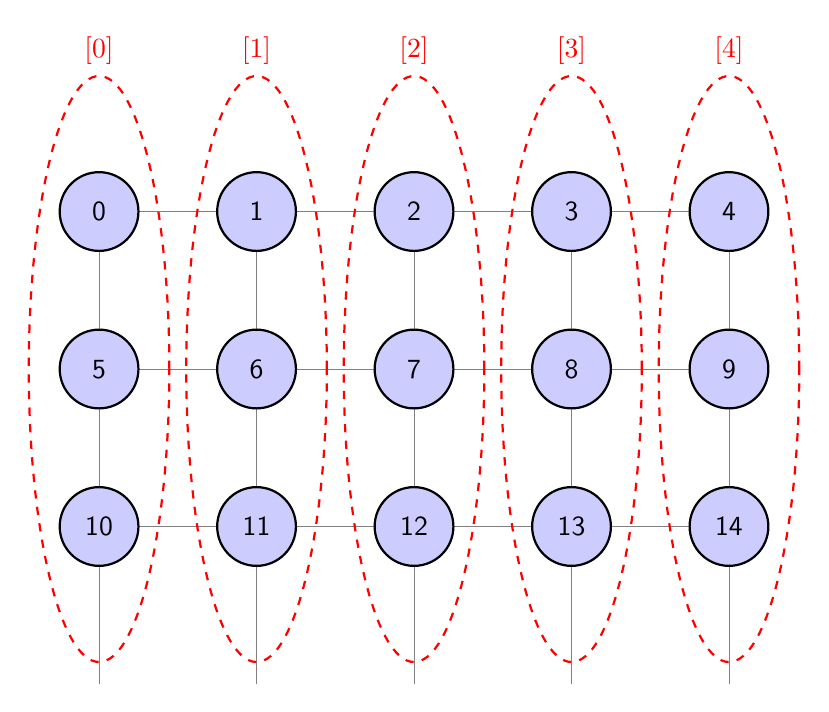
\begin{tikzpicture}[>=Stealth, thick, node distance=2 cm]
	% Styles for different components
	\tikzset{
		main node/.style={circle, draw, fill=blue!20, minimum size=1cm, font=\sffamily},
		class node/.style={dashed, thick, ellipse, draw, thick, red, minimum height=1cm, minimum width=1cm, align=center},
		path/.style={->, thick, shorten <=2pt, shorten >=2pt},
		reflexive/.style={->, line width=1mm, loop, looseness=5, in=0, out=-90, red, opacity=.5},
		symmetric/.style={->, line width=1mm, blue, bend left, opacity=.5},
		transitive/.style={->, thick, green!75!black, bend left}
		label distance=3mm
	}
	
	% Nodes representing elements
	\node[main node] (0) {0};
	\node[main node] (1) [right of=0] {1};
	\node[main node] (2) [right of=1] {2};
	\node[main node] (3) [right of=2] {3};
	\node[main node] (4) [right of=3] {4};
	
	\node[main node] (5) [below of=0] {5};
	\node[main node] (6) [below of=1] {6};
	\node[main node] (7) [below of=2] {7};
	\node[main node] (8) [below of=3] {8};
	\node[main node] (9) [below of=4] {9};
	
	\node[main node] (10) [below of=5] {10};
	\node[main node] (11) [below of=6] {11};
	\node[main node] (12) [below of=7] {12};
	\node[main node] (13) [below of=8] {13};
	\node[main node] (14) [below of=9] {14};
	
%	\foreach \x in {0,1,2,...,14} {
%		\draw[reflexive] (\x) to (\x);
%	}
%	
%	\foreach \x/\y in {
%		0/5, 5/10, 1/6, 6/11,
%		2/7, 7/12, 3/8, 8/13,
%		4/9, 9/14} {
%		\draw[symmetric] (\x) to (\y);
%		\draw[symmetric] (\y) to (\x);
%	}
%	
%	\foreach \a/\b in {
%		0/10, 1/11, 2/12, 3/13, 4/14} {
%		\draw[->, line width=1mm, green!75!black, bend left=20pt, opacity=.5] (\a) to (\b);
%		\draw[->, line width=1mm, green!75!black, bend left=20pt, opacity=.5] (\b) to (\a);
%	}
	
	%	 Nodes for equivalence classes
	\node[class node, label={[red]above:$[0]$}, fit=(0) (5) (10)] {};
	\node[class node, label={[red]above:$[1]$}, fit=(1) (6) (11)] {};
	\node[class node, label={[red]above:$[2]$}, fit=(2) (7) (12)] {};
	\node[class node, label={[red]above:$[3]$}, fit=(3) (8) (13)] {};
	\node[class node, label={[red]above:$[4]$}, fit=(4) (9) (14)] {};
%	\node[class node, label={[red]above:Class $[2, 3]$}, fit=(2) (3)] {};
%	\node[class node, label={[red]above:Class $[4, 5]$}, fit=(4) (5)] {};
	
	
	% Background grid as optional visual enhancement
	\begin{scope}[on background layer]
		\draw[style=help lines, step=2cm] (0,0) grid (8,-6);
	\end{scope}
\end{tikzpicture}}
\end{minipage}
\end{center}

\section*{Quotient Sets}
\begin{center}
\adjustbox{scale=.9}{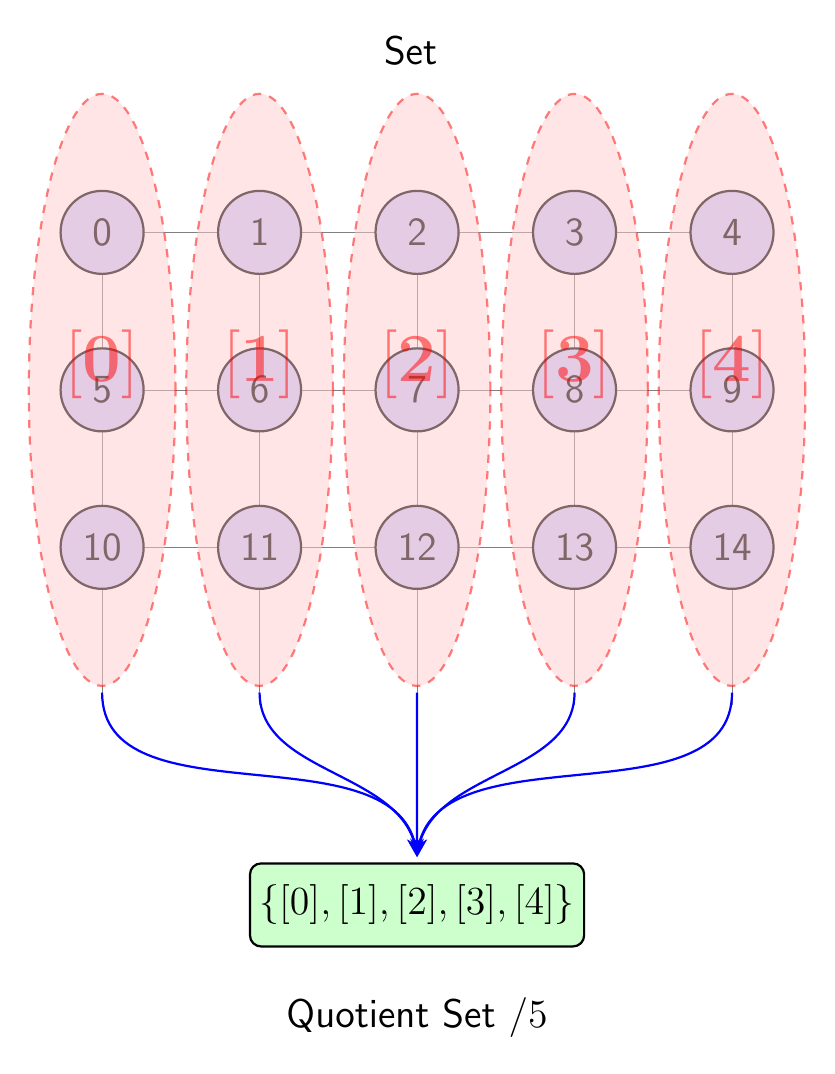
\begin{tikzpicture}[>=Stealth, thick, node distance=2cm, auto]
	% Styles
	\tikzset{
		main node/.style={circle, draw, fill=blue!20, minimum size=30pt, font=\sffamily\Large},
		class node/.style={dashed, ellipse, draw, thick, red, fill=red!20, minimum height=1cm, minimum width=1cm, align=center, opacity=.5}, % drop shadow
		quotient node/.style={rectangle, draw, thick, fill=green!20, minimum size=30pt, font=\sffamily\Large, rounded corners},
		path/.style={blue,->, thick, shorten <=2pt, shorten >=2pt, decorate},
		%decoration={snake, amplitude=.4mm, segment length=2mm, post length=1mm}
		label distance=2mm
	}
	
	% Nodes representing elements of the set% Nodes representing elements
	\node[main node] (0) {0};
	\node[main node] (1) [right of=0] {1};
	\node[main node] (2) [right of=1] {2};
	\node[main node] (3) [right of=2] {3};
	\node[main node] (4) [right of=3] {4};
	
	\node[main node] (5) [below of=0] {5};
	\node[main node] (6) [below of=1] {6};
	\node[main node] (7) [below of=2] {7};
	\node[main node] (8) [below of=3] {8};
	\node[main node] (9) [below of=4] {9};
	
	\node[main node] (10) [below of=5] {10};
	\node[main node] (11) [below of=6] {11};
	\node[main node] (12) [below of=7] {12};
	\node[main node] (13) [below of=8] {13};
	\node[main node] (14) [below of=9] {14};
	
%	% Nodes for equivalence classes
	\node[class node, fit=(0) (5) (10)] (class0) {\Huge $\mathbf{[0]}$};
	\node[class node, fit=(1) (6) (11)] (class1) {\Huge $\mathbf{[1]}$};
	\node[class node, fit=(2) (7) (12)] (class2) {\Huge $\mathbf{[2]}$};
	\node[class node, fit=(3) (8) (13)] (class3) {\Huge $\mathbf{[3]}$};
	\node[class node, fit=(4) (9) (14)] (class4) {\Huge $\mathbf{[4]}$};
	
%	% Quotient set nodes
	\node[quotient node, below=4cm of $(11)!0.5!(13)$] (qset) {$\{[0], [1], [2], [3], [4]\}$};
%	
%	% Paths for quotient set formation
	\draw[path] (class0) to[out=-90, in=90] (qset);
	\draw[path] (class1) to[out=-90, in=90] (qset);
	\draw[path] (class2) to[out=-90, in=90] (qset);
	\draw[path] (class3) to[out=-90, in=90] (qset);
	\draw[path] (class4) to[out=-90, in=90] (qset);
%	
%	% Annotations and decorative lines
	\node[align=center, above=2cm of $(1)!0.5!(3)$, font=\sffamily\Large] {Set $\Z$};
	\node[align=center, below=0.5cm of qset, font=\sffamily\Large] {Quotient Set $\Z/5\Z$};
	
	% Background grid
	\begin{scope}[on background layer]
		\draw[style=help lines, step=2cm, gray, very thin] (0,0) grid (8,-6);
	\end{scope}
\end{tikzpicture}}
\end{center}


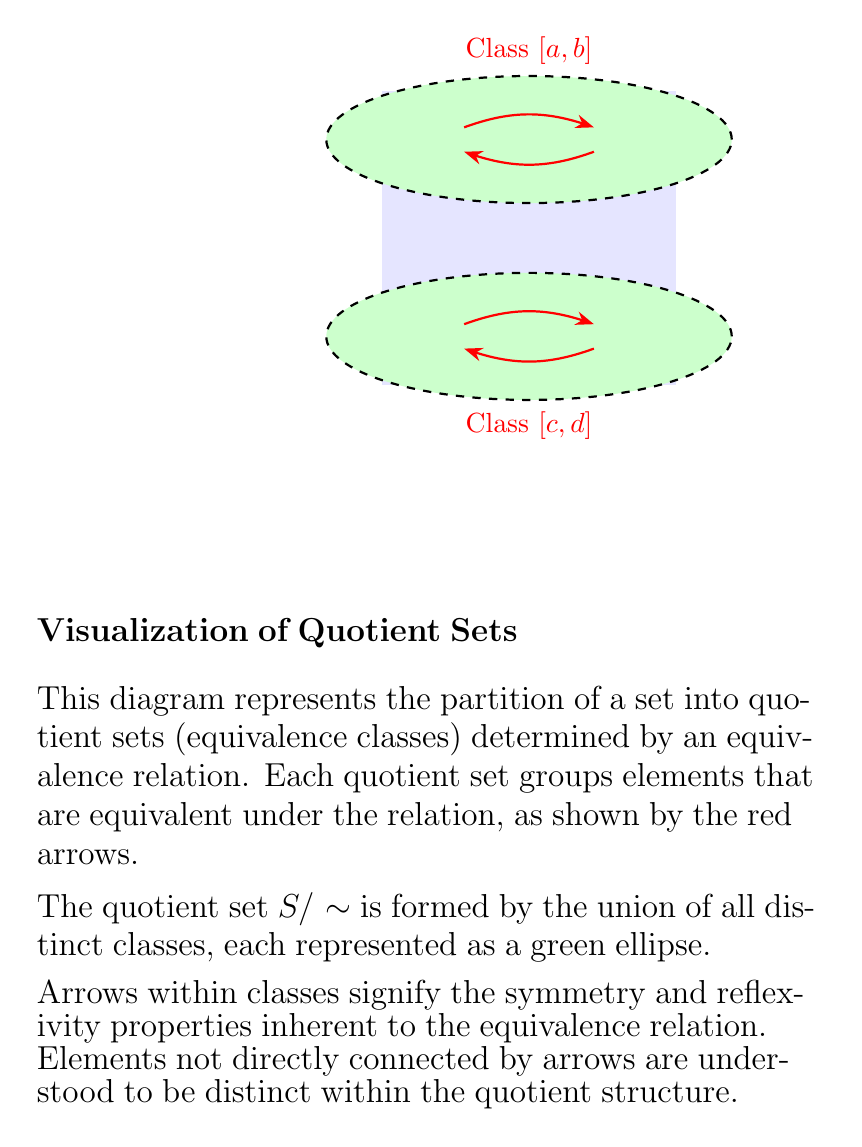
\begin{tikzpicture}[>=Stealth, thick, node distance=2.5 cm]
	% Styles for different elements and classes
	\tikzset{
		main node/.style={circle, draw, fill=blue!30, thick, minimum size=25pt, inner sep=0pt},
		class node/.style={ellipse, draw, thick, dashed, fill=green!20, minimum width=3cm, minimum height=1.5cm},
		path/.style={->, thick, shorten <=2pt, shorten >=2pt},
		relation/.style={->, thick, bend left=20, red},
		class label/.style={color=red, align=center}
	}
	
	% Nodes representing elements
	\node[main node] (a) {a};
	\node[main node] (b) [right of=a] {b};
	\node[main node] (c) [below of=a] {c};
	\node[main node] (d) [right of=c] {d};
	
	% Class node
	\node[class node, fit=(a) (b), label={[class label]above:Class $[a, b]$}] {};
	\node[class node, fit=(c) (d), label={[class label]below:Class $[c, d]$}] {};
	
	% Relations indicating equivalence
	\draw[relation] (a) to (b);
	\draw[relation] (b) to (a);
	\draw[relation] (c) to (d);
	\draw[relation] (d) to (c);
	
	% Annotations
	\node[align=left, text width=10cm, below=3cm of c] {
		\large \textbf{Visualization of Quotient Sets}\\[2ex]
		This diagram represents the partition of a set into quotient sets (equivalence classes) determined by an equivalence relation. Each quotient set groups elements that are equivalent under the relation, as shown by the red arrows.\\[1ex]
		The quotient set $S/\sim$ is formed by the union of all distinct classes, each represented as a green ellipse.\\[1ex]
		Arrows within classes signify the symmetry and reflexivity properties inherent to the equivalence relation. Elements not directly connected by arrows are understood to be distinct within the quotient structure.
	};
	
	% Optional background for quotient set
	\begin{scope}[on background layer]
		\fill[blue!10] ($(a.north west)+(-0.3,0.3)$) rectangle ($(d.south east)+(0.3,-0.3)$);
	\end{scope}
\end{tikzpicture}\ \\
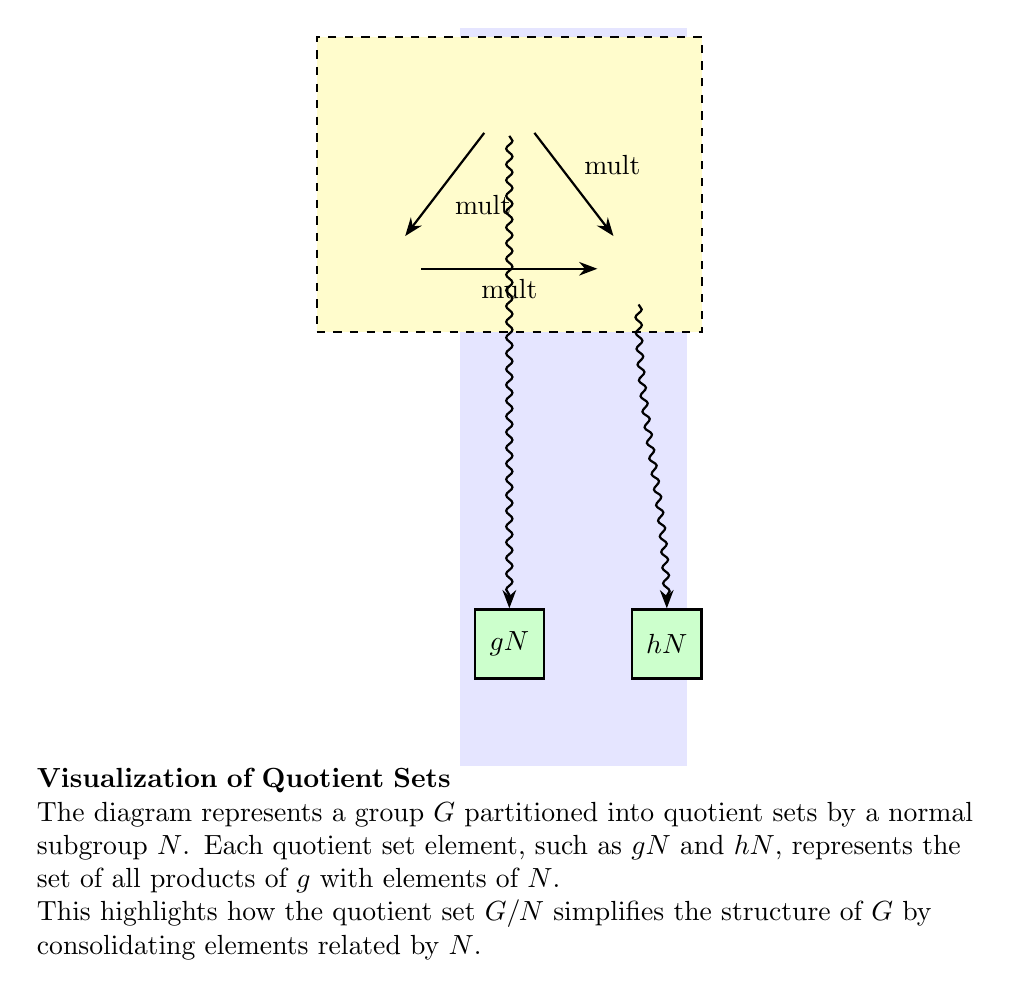
\begin{tikzpicture}[>=Stealth, thick, node distance=2 cm, auto]
	% Styles
	\tikzset{
		main node/.style={circle, draw, fill=blue!20, thick, minimum size=25pt, font=\sffamily\bfseries},
		subgroup node/.style={circle, draw, fill=red!30, thick, minimum size=25pt, font=\sffamily\bfseries},
		quotient node/.style={rectangle, draw, fill=green!20, thick, minimum size=25pt, align=center},
		path/.style={->, thick, shorten <=2pt, shorten >=2pt},
		group/.style={draw, dashed, fill=yellow!20, inner sep=10pt}
	}
	
	% Nodes for group elements
	\node[main node] (g) {g};
	\node[subgroup node] (n) [below left=1.5cm and 1cm of g] {n};
	\node[main node] (h) [below right=1.5cm and 1cm of g] {h};
	
	% Nodes for quotient set elements
	\node[quotient node] (gN) [below=6cm of g] {\(gN\)};
	\node[quotient node] (hN) [right of=gN] {\(hN\)};
	
	% Dashed group boundary
	\node[group, fit=(g) (n) (h)] (group) {};
	
	% Paths
	\draw[path] (g) -- node {mult} (n);
	\draw[path] (g) -- node {mult} (h);
	\draw[path] (n) -- node [swap] {mult} (h);
	
	% Mapping to quotient set
	\draw[->, thick, decorate, decoration={snake, amplitude=.4mm, segment length=2mm, post length=1mm}] 
	(g) to[out=-90, in=90] (gN);
	\draw[->, thick, decorate, decoration={snake, amplitude=.4mm, segment length=2mm, post length=1mm}] 
	(h) to[out=-90, in=90] (hN);
	
	% Annotations
	\node[align=left, text width=12cm, below=1cm of gN] {
		\textbf{Visualization of Quotient Sets}\\
		The diagram represents a group \(G\) partitioned into quotient sets by a normal subgroup \(N\). Each quotient set element, such as \(gN\) and \(hN\), represents the set of all products of \(g\) with elements of \(N\).\\
		This highlights how the quotient set \(G/N\) simplifies the structure of \(G\) by consolidating elements related by \(N\).
	};
	
	% Background shading for quotient set
	\begin{scope}[on background layer]
		\fill[blue!10] ($(g.north west)+(-0.3,0.6)$) rectangle ($(h.south east)+(0.3,-6)$);
	\end{scope}
\end{tikzpicture}

\newpage
%\begin{tikzpicture}[scale=1.5]
%	
%	% Draw the outer circle representing group G
%	\draw[thick] (0,0) circle (3cm);
%	\node at (0,3.2) {$G$};
%	
%	% Draw the inner circle representing the normal subgroup N
%	\draw[thick] (0,0) circle (1.5cm);
%	\node at (0,1.7) {$N$};
%	
%	% Draw elements of G
%	\foreach \angle in {0,45,...,315}
%%	\filldraw (3cm*\angle:1pt) circle (2pt);
%	
%	% Draw elements of N
%	\foreach \angle in {0,90,...,270}
%	\filldraw (1.5cm*\angle:1pt) circle (2pt);
%	
%	% Draw arrows indicating normal subgroup property
%%	\foreach \angle in {0,90,...,270} {
%%		\draw[->,thick] (1.5cm*\angle:1.5cm) -- (3cm*\angle:3cm);
%%		\draw[->,thick] (3cm*\angle:3cm) -- (1.5cm*\angle:1.5cm);
%%	}
%	
%	% Draw label for G and N
%	\node at (0,0) {$e$};
%	
%	% Draw cosets
%	\node at (1.5, 0) {$gN$};
%	\node at (-1.5, 0) {$hN$};
%	
%\end{tikzpicture}
%\input{acp-note-bib}
\end{document}
